\documentclass[10pt,a4paper]{article}
\usepackage[latin1]{inputenc}
\usepackage{amsmath}
\usepackage{amsfonts}
\usepackage{amssymb}
\usepackage{graphicx}
\usepackage{float}
\usepackage{soul}
\usepackage{caption}
\usepackage{subcaption}
\usepackage[section]{placeins}
\usepackage[left=2cm,right=2cm,top=2cm,bottom=2cm]{geometry}
\author{Akshat Mahajan}
\title{Physics 180Q - Lab Report 5}
\begin{document}
\maketitle

\noindent \textsl{This lab was performed in conjunction with Hanwen Qin. The variable impedance terminator was set to 10 k$\Omega$ throughout, as analysis of the results from Week 1 had demonstrated that it gave the most accurate responses overall. On Friday evening and Sunday, I worked with a variable impedance of 50 k$\Omega$ in order to avoid disturbing the Friday lab's successful setup.}\\
\\
The goal of this lab was to build an optical cavity; photograph higher-order modes of the laser beam and test out predictions regarding the cavity finesse and linewidth. We also attempted to mode-match cavities.\\
\\
During the regular lab session on Thursday, we were able to partially meet these objectives. I spent an additional thirteen hours following this attempt to fulfill the other goals while working by myself, but was mostly unsuccessful. What few results I was able to obtain I will present here, alongside our original results.\\
\\Important equations used throughout:

$$R(z) = z\left(1 + \dfrac{z_{0}^{2}}{z^{2}}\right)$$
$$w_{z}^{2} = w_{0}^{2}\left(1 + \dfrac{z^{2}}{z_{0}^{2}}\right)$$
$$q(z) = \dfrac{1}{R(z)} - i\dfrac{\lambda}{n\pi w(z)^{2}}$$

These are respectively the radius, waist and quality factor equation. Here, $w_{0}$ is the minimum waist of the beam and $z_{0}$ is a constant dependent on the minimum waist.

\section*{Part 1: Beam Waist and Quality Factor Measurements Measurements}


We were provided a pre-determined setup with which to work with. A 10 mV (3.334 mW) laser with an attenuator was focused and allowed to impinge on a single-mode optical fiber coupling some distance away. \\
\\
Initially, we assumed that the fiber coupling was already at its maximum efficiency, and worked with the existing power coming through the beam, approximately 0.06 mW. In retrospect, this corresponded to a 1.8\% efficiency. On Friday and Sunday, however, I worked with a 4.4 mV (1.46 mW) beam, realizing a coupling efficiency of about 44\%.\\
\\
We proceeded to measure the minimum waist purely in the $x$-direction by fitting the waists obtained at three separate distances to the power distribution:$$P(z) = \dfrac{P}{2}\left(1 \pm \mathrm{erf}\left(\sqrt{2}\dfrac{x}{w_{x}}\right)\right)$$ The $\pm$ sign ambiguity arises because we are translating a knife-edge across the beam, and we have the freedom to choose whether the knife advances along the positive $x$ or negative $x$ direction.\\
\\
On Thursday, we chose distances of 72 mm, 390 mm and 890 mm respectively, using the end of the fiber coupling as our reference point for distances. On Friday, I chose distances of 150, 260, and 495 mm, again using the end of the fiber coupling as the reference point for distances. Our background corrections for the power was 2.6 mV (8.66 $\mu$W) with the lights off on Thursday at about 200 mV/div, and 5 mV on Thursday at 5 volts/division on the oscilloscope.\\
\\
Our initial results were not promising, and could not be explained using the standard theoretical distribution.
\begin{table}[H]
\centering
\begin{tabular}{|c|c|}
 \hline 
 Distance(mm) & Waists (mm) \\ 
 \hline 
 97 & 0.558 \\ 
 \hline 
 473 & 0.588 \\
 \hline
 890 & 0.534\\
 \hline
 \end{tabular}
\caption{Initial waist measurements on Thursday}
\end{table}
As can be seen from the data, our waist measurements surprisingly included an apparent \textsl{maximum} rather than a minimum. This is not in line with the theoretical waist equation.\\
\\
\textbf{We repeated these measurements but obtained the same result}. A problem with our fits may be ruled out through examination of the profiles in Figure 1. Interestingly, our nonlinear fits to the waist equation were still able to discern meaningful results. 
\begin{figure}[H]
\centering
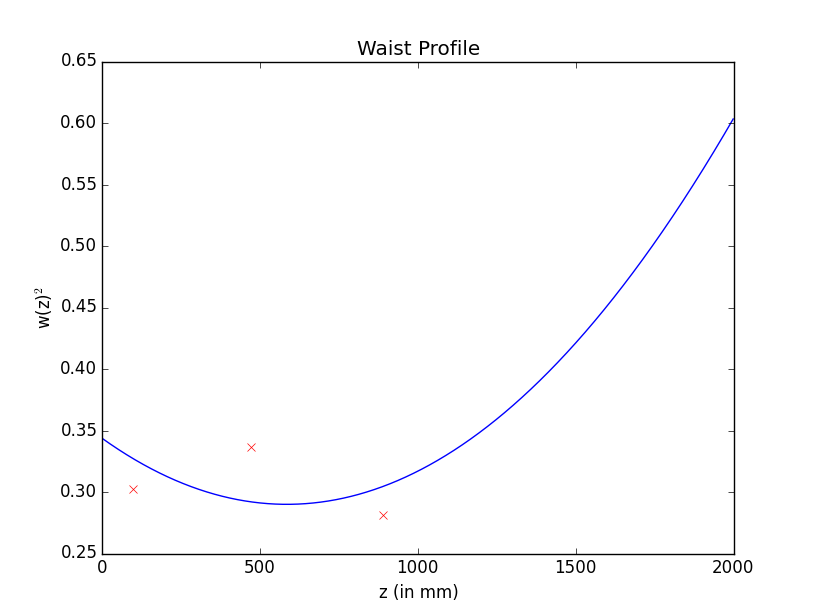
\includegraphics[scale=0.5]{../Analysis/thursday_waist_fit.png}
\caption{Nonlinear fit to the minimum waist equation on Thursday}
\end{figure}
\begin{figure}[t]
\centering
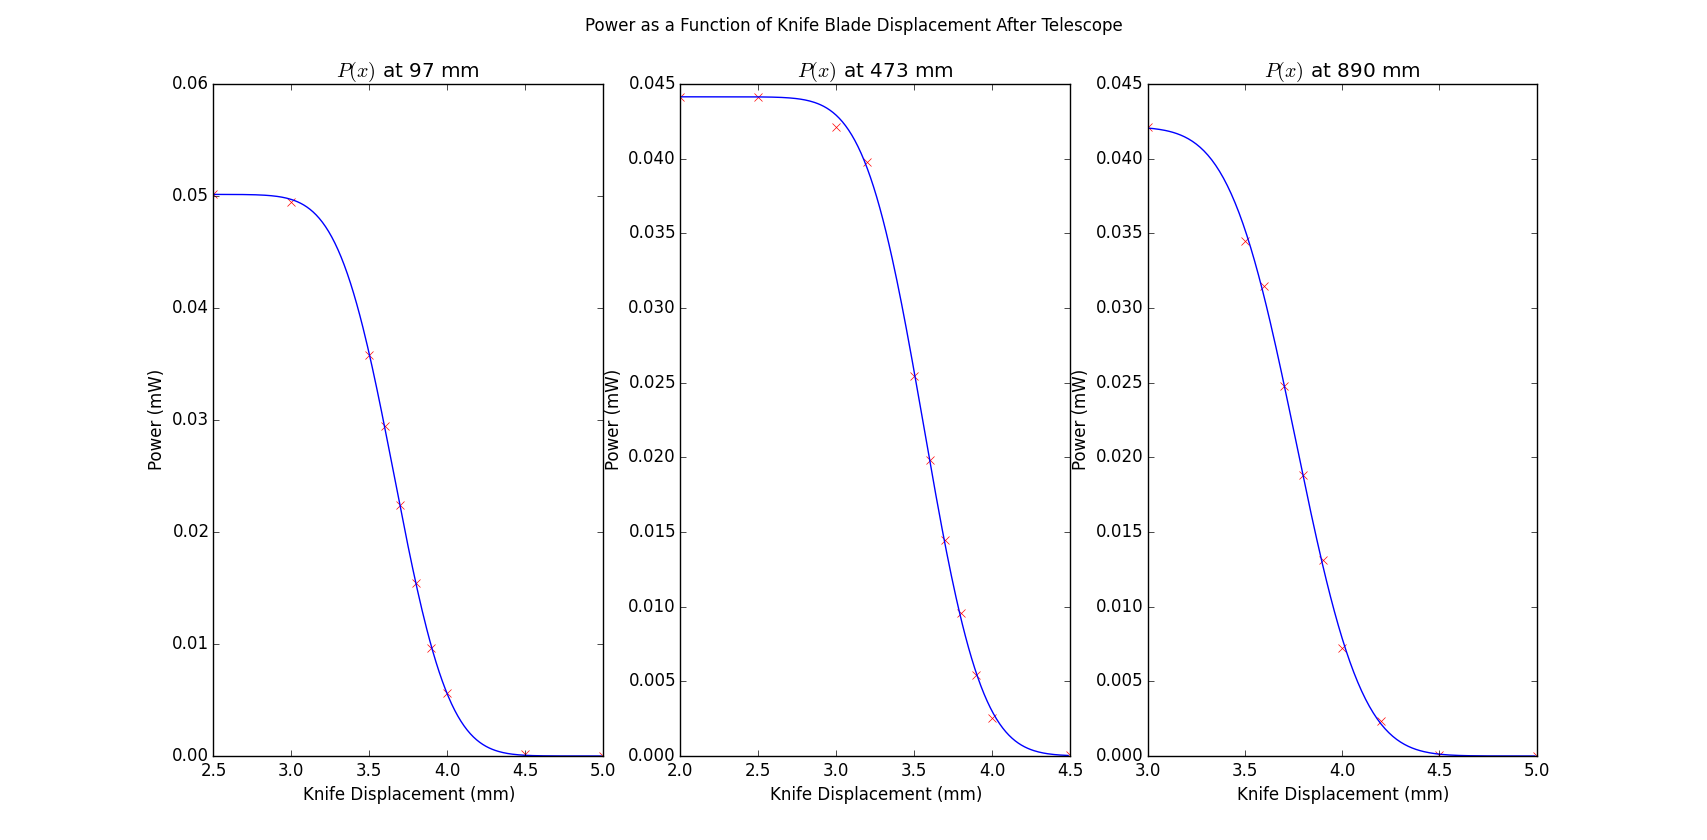
\includegraphics[scale=0.4]{../Analysis/thursday_waists.png}
\caption{Fitting to the power law distribution on Thursday}
\end{figure}
\noindent The minimum waist on Thursday was found to be 0.529 mm at a distance of approximately 586 mm - Hanwen's program, however, led us to believe that that the true minimum was obtained at 629 mm. The beam's quality factor can then be estimated (using Hanwen's results) just before the minimum waist as $$q(628\;\mathrm{mm}) = 1.577\times 10^{-12} -7.1i\times10^{-3}$$
\noindent On Friday, the results obtained were markedly improved. 
\begin{table}[H]
\centering
\begin{tabular}{|c|c|}
 \hline 
 Distance(mm) & Waists (mm) \\ 
 \hline 
 150 & 0.510 \\ 
 \hline 
 260 & 0.428 \\
 \hline
 495 & 0.316\\
 \hline
 \end{tabular}
\caption{Initial waist measurements on Friday}
\end{table}
\begin{figure}[H]
\centering
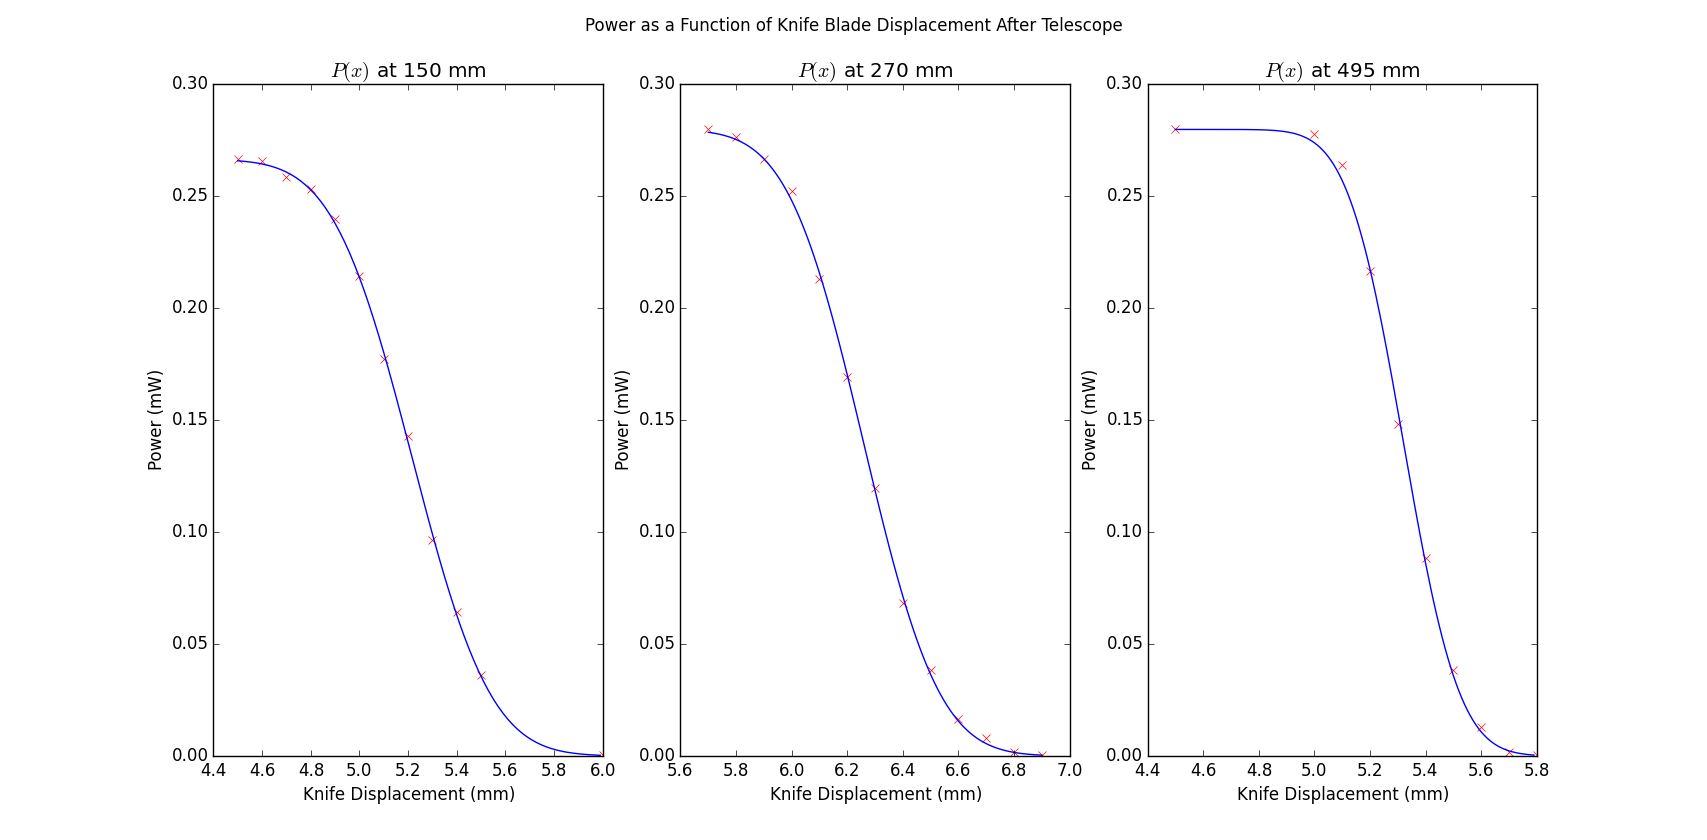
\includegraphics[scale=0.4]{../Analysis/friday_waists.png}
\caption{Fitting to the power law distribution on Friday} 
\end{figure}
\begin{figure}[H]
\centering
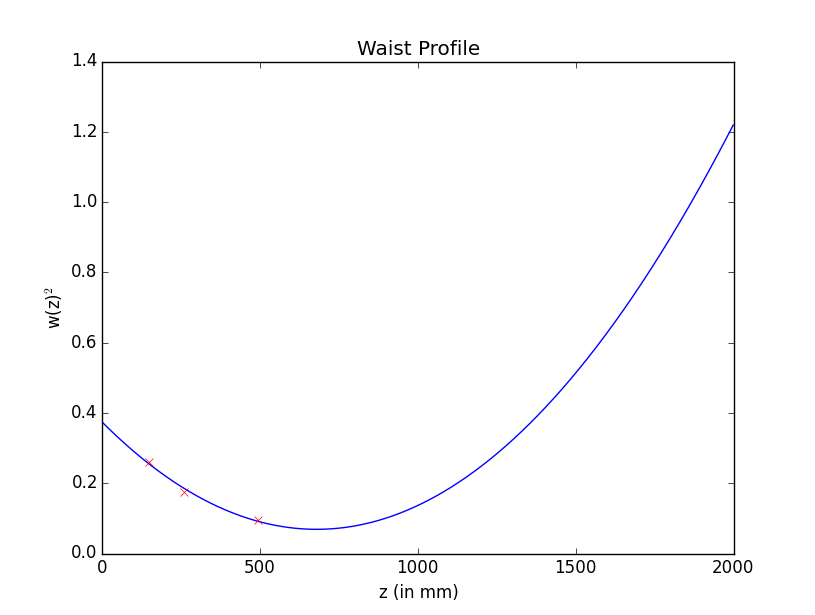
\includegraphics[scale=0.5]{../Analysis/friday_waists_fit.png}
\caption{Nonlinear fit to the minimum waist equation on Friday}
\end{figure}
\noindent This time the minimum was found to be 0.06 mm and at 680 mm. Our quality factor just before the minimum waist is then $$q(679\;\mathrm{mm}) = 7.85\times 10^{-9} -5.9i\times10^{-2}$$
\section*{Part 2: Cavity Measurements}
Let's let $L$ be the total length that light travels in one unit cell of our optical cavity. Let $d_{1}, d_{2}$ be the dimensions of the optical cavity, with $d_{1} > d_{2}$ and $d_{1}$ the distance from the input mirror to the second mirror. Then $L = 2d_{1} + 2\sqrt{d_{1}^{2} + d_{2}^{2}}$. We also use $R$ as the radius of curvature of our concave mirror in our bowtie cavity.\\
\\
The T-matrix of our system can be worked out as 

$$T = \begin{pmatrix}
1 & \frac{L}{2}\\
0 & 1
\end{pmatrix}\begin{pmatrix}
1 & 0\\
-\frac{2}{R} & 1
\end{pmatrix}\begin{pmatrix}
1 & \frac{L}{2}\\
0 & 1
\end{pmatrix} = \begin{pmatrix}
1 & \frac{L}{2}\\
0 & 1
\end{pmatrix}\begin{pmatrix}
1 & \frac{L}{2}\\
-\frac{2}{R} & 1 - \frac{L}{R}
\end{pmatrix} = \begin{pmatrix}
1 - \frac{L}{R} & L - \frac{L^{2}}{2R}\\
-\frac{2}{R} & 1 - \frac{L}{R}
\end{pmatrix}
$$
Stability requires that $$-1 \leq 1 - \frac{L}{R} \leq 1$$ i.e as long as $0 \leq L \leq 2R$, our cavity will be stable. Here\footnote{This can be seen from the Newport concave lens manual}, $R = 1\;\mathrm{m}$, so we have near-complete freedom in choosing our dimensions so that they do not exceed 2 m.\\
\\
\textbf{For our design, we took $d_{1}$ = 10 inches or 25.4 centimetres, and $d_{2}$ = 3 inches or 7.62 centimetres.} The stability condition is well met; we see that our $L = 103.83$ cm or just about 1 m.\\
\\
\textbf{The same setup was employed on Friday/Sunday}. We chose the following arrangement:
\begin{itemize}
\item First (input) mirror $\longrightarrow$ PF10-03-P01P (Thorlabs)
\item Second (output) mirror $\longrightarrow$ PF10-03-P01P (Thorlabs)
\item Curved mirror $\longrightarrow$ 10DC1000ER.2 (Newport)
\item Fourth mirror $\longrightarrow$ BB1-E02P (Thorlabs)
\end{itemize}
Via a brute-force search through all possible lenses, it was determined that the best possible mode-matching lens combination was obtained with a telescope with objective of focal length 53 mm and eyepiece of focal length 30 mm.\\
\\
We proceeded to align the cavity as best as possible without the use of mode-matching lenses. On Thursday, this was not possible, owing to the low power input to the cavity in the first place - no signal discernible from background noise was consequently observed through the output mirror. On Friday/Sunday, however, a \textbf{very} small signal (approximately 200 $\mu$V or 6.668 $\mu$W) was observable (but only after changing the volts/div from 5 volts/div to 200 mV/div) - this signal fluctuated rapidly, and building a small cardboard house around the optical cavity did not diminish the variability. This was after extensive cavity alignment resulted in a maximised, noticeable signal.\\
\\
On Thursday, we placed a camera and observed the following higher-order modes\footnote{This was not done on Friday/Sunday for three reasons: 1) so as to save time, 2) the camera could not be found in the lab (shockingly), 3) I finally decided to stop looking for the camera and go eat, following which I lost my beautiful coupling efficiency, making the lack of a camera the least of my worries.}
\begin{figure}[H]
\centering
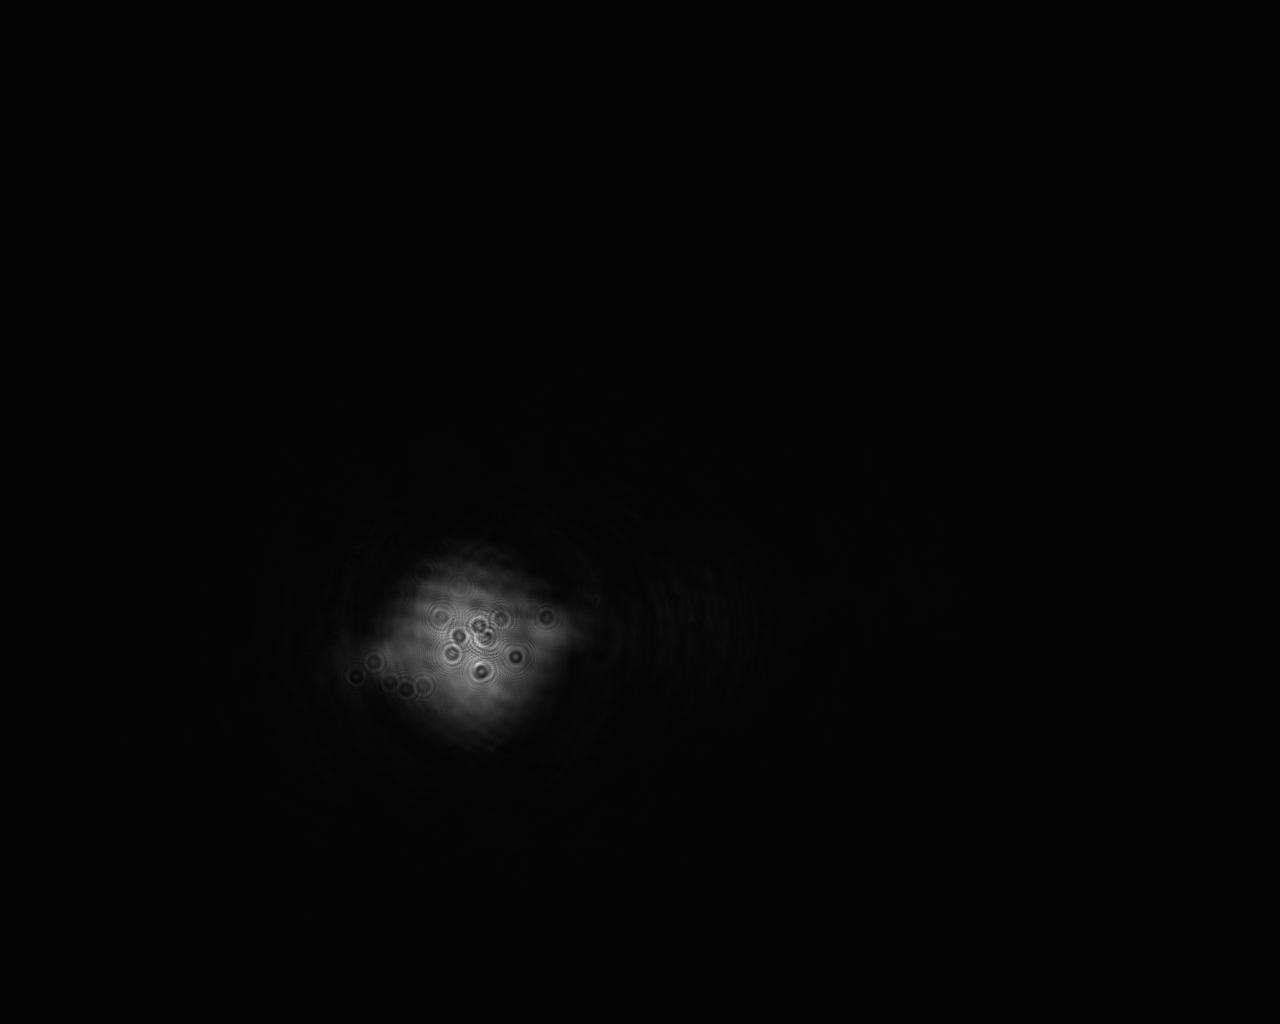
\includegraphics[width=\textwidth]{../Analysis/Lab5Mode8.png}
\caption{A first-order mode}
\end{figure}
\begin{figure}[H]
\centering
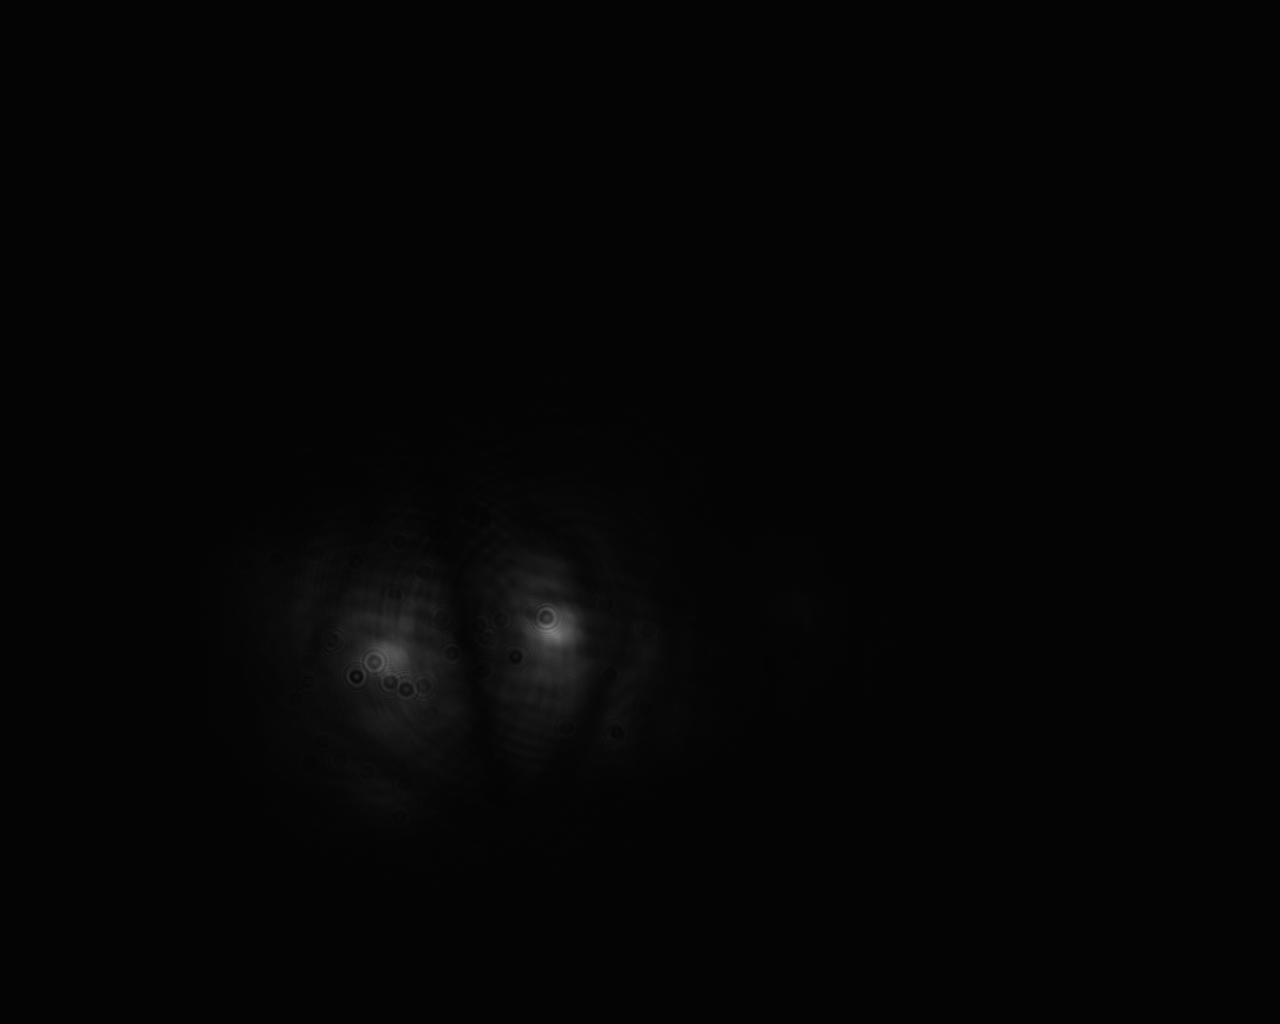
\includegraphics[width=\textwidth]{../Analysis/Lab5Mode7.png}
\caption{A second-order mode}
\end{figure}
\begin{figure}[H]
\centering
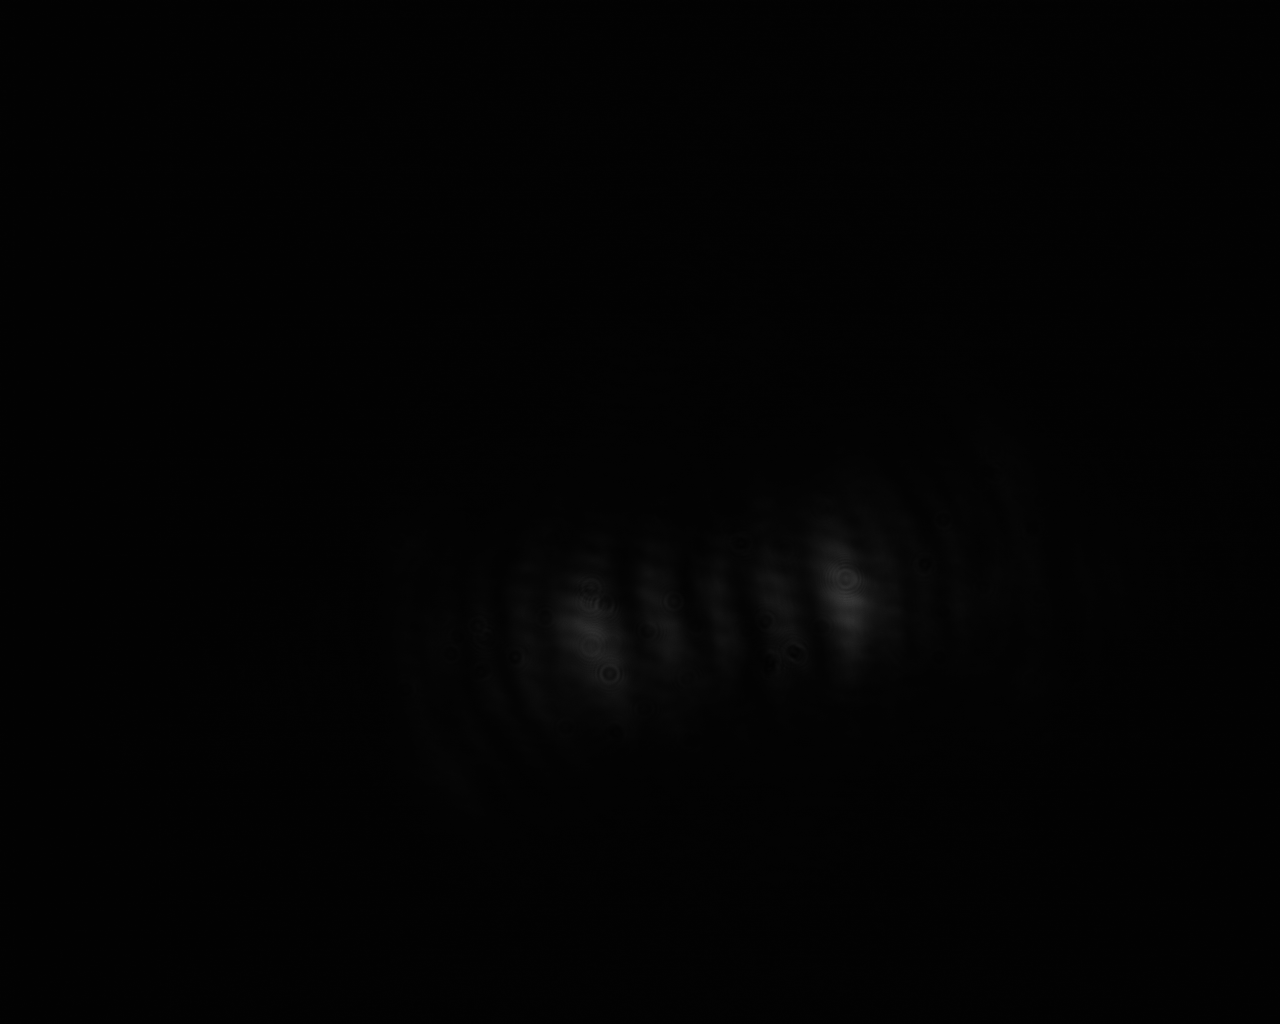
\includegraphics[width=\textwidth]{../Analysis/Lab5Mode2.png} 
\caption{A fifth-order mode}
\end{figure}
\begin{figure}[H]
\centering
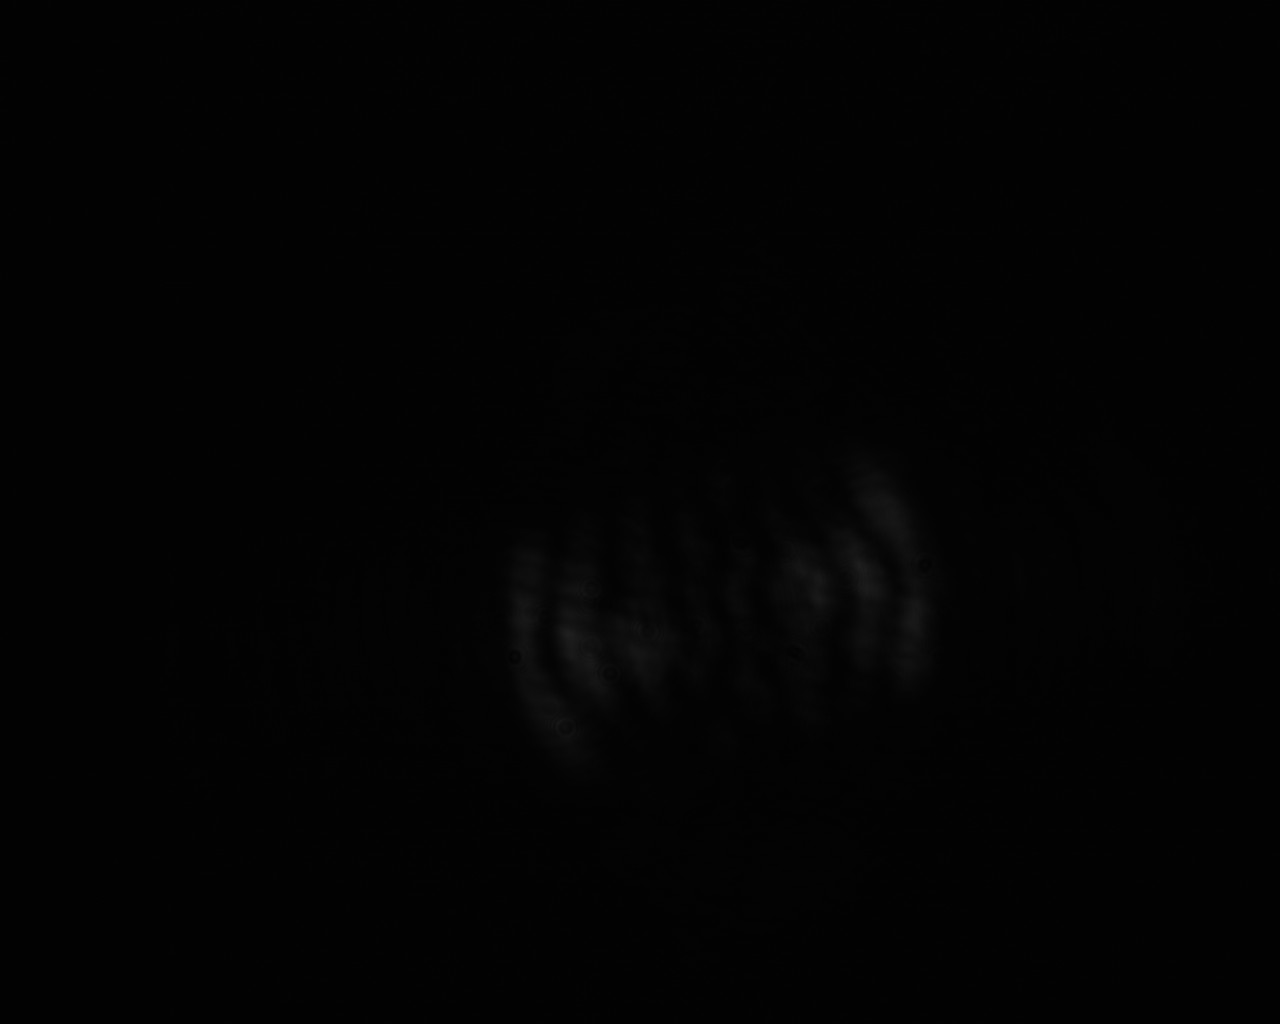
\includegraphics[width=\textwidth]{../Analysis/Lab5Mode3.png}
\caption{A sixth-order mode}
\end{figure} 
\begin{figure}[H]
\centering
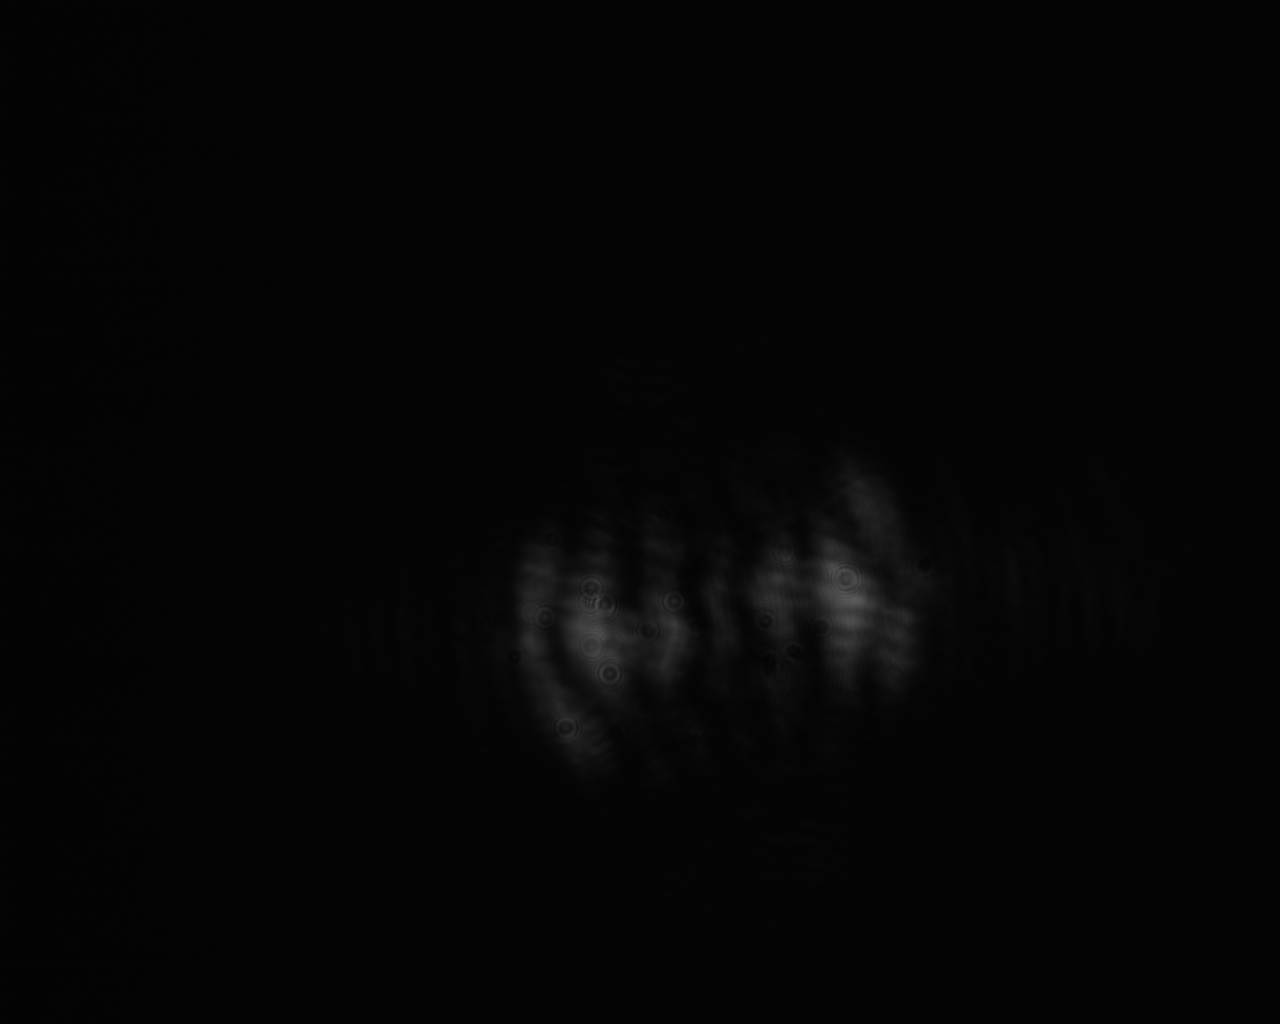
\includegraphics[width=\textwidth]{../Analysis/Lab5Mode1.png}
\caption{A seventh-order mode}
\end{figure}
\section*{Part 3: Scanning the Cavity}
We proceeded to hook up our concave mirror (mounted on the mirror mount with wires attached to it) and to scan the cavity with Justin's help on Thursday. However, due to low signal quality, no discernible effect was seen in the signal.\\
\\
On Friday/Sunday, the same thing happened. The low power through the optical cavity and high volatility yielded no discernible measurements. \textbf{The cavity linewidth and finesse could not be recorded.}
\section*{Part 5: Mode Matching}
We know that the cavity waist can be determined as 
$$ w(0)^{2} = \lambda\dfrac{L - \frac{L^{2}}{2R}}{\pi\sqrt{1 - \left(1 - \frac{L}{R}\right)^{2}}} \approx \dfrac{\lambda}{2\pi} = 106\;\mathrm{nm}$$
where we have used the approximation of $L = R = 1$ m. It is important to note that the minimum cavity waist is taken to occur at the beginning of the optical cavity. The radius of the optical cavity vanishes at the minimum cavity waist i.e. $R \leftarrow \infty$ . Our laser beam wavelength $\lambda$ was taken to be 670 nm, meaning our cavity waist is about 1.29 $\times$ 10$^{-4}$m or just 0.129 mm.\\
\\
On Thursday, the laser beam coincided with the optical cavity at 695 mm from the laser collimator. We placed our telescope at 195 mm from the laser collimator. Our resulting beam at the start of the waist on Thursday (taking Hanwen's claim that the true minimum occured at 629 mm) therefore came out to comprise of $w = 0.140$mm and $R = 417$ mm - in other words, close to the cavity waist. Similar measurements ($w = 0.142$mm and $R = 417$ mm) were obtained if the true minimum of the beam was taken to be at 586 mm (according to my calculations).\\
\\
On Sunday, the telescope system was taken to be at 100 mm from the laser head. This time around, the cavity waist was 0.115 mm while the radius of curvature was much larger than before, at about 487 mm, so the system could be said to better match the cavity quality factor on Sunday, if not the cavity waist itself.\\
\\
However, owing to the low signal quality through the cavity, no distinct power output occurred on Sunday or Thursday\footnote{Sunday was particularly unfavourable owing to the lost coupling efficiency.}. Thus, \textbf{the mode matching experiment could not be completed.}
\end{document}